\paragraph{Слои модели}

Наконец, после успешного размещения модель разбивается на слои,
представляющие различные структурные элементы здания,
например стены, окна или лестницы. На любой выделенный слой
можно накладывать эффект отображения, как это описывалось
в разделе~\ref{subsections:ClientServerDesign}.
Для разбиения модели на слои реализуется вспомогательный класс
\emph{LayerController}, чей принцип работы показан
на схеме~\ref{figure:SInitLayers}.

\begin{figure}[!htp]
    \centering
    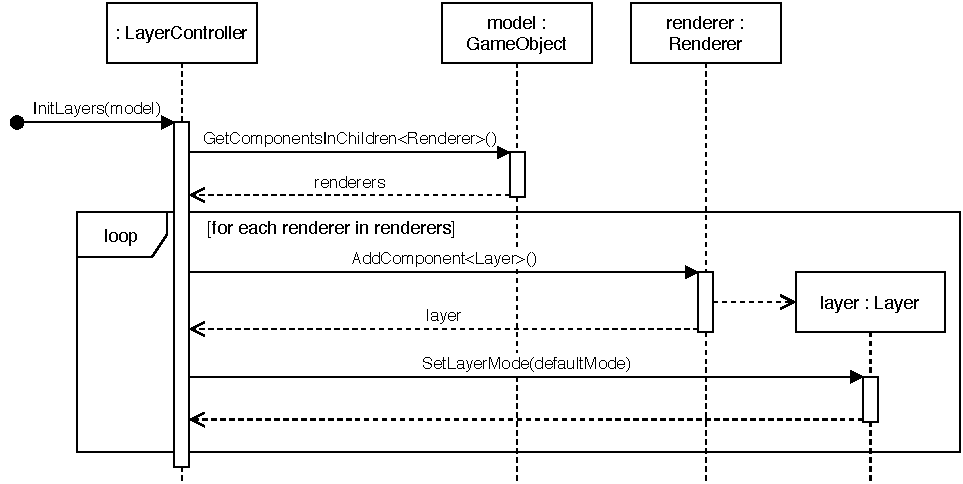
\includegraphics[width=0.9\textwidth]{images/UML-SInitLayers.pdf}
    \caption{Разбиение модели на слои.}
    \label{figure:SInitLayers}
\end{figure}

Слои модели были реализованы с помощью компонента \emph{Layer}.
Для разбиения на слои можно воспользоваться тем фактом,
что при экспорте модель проходила процесс статического батчинга
(разделы \ref{subsections:Optimization} и \ref{subsections:ServerImpl}),
тем самым каждый потенциальный слой модели имеет свой компонент \emph{Renderer},
отвечающий за отрисовку, и является дочерним по отношению к самой модели.
Следовательно, каждый такой объект можно рассматривать как слой модели.
После разбиения каждому слою модели может быть назначен
свой режим отображения, как показано на рисунке~\ref{figure:SLayerSetMode}.

\begin{figure}[!htp]
    \centering
    \includegraphics[width=0.6\textwidth]{example-image}
    \caption{Изменение режима отображения слоя модели.}
    \label{figure:SLayerSetMode}
    \comment{Layer.SetLayerMode вместо Layer.Current}
\end{figure}

\intextcomment{
    Описание UML\dots
}
Всего в рамках прототипа было реализовано 4 режима отображения:

\begin{itemize}
    \item {
        ``Стандартный''

        Стандартный режим не имеет какого-либо особого поведения и
        демонстрирует слой в том виде, в котором он изначально задумывался.
    }
    \item {
        ``Невидимый''

        Невидимый режим отключает отображение через отключение активности слоя.
    }
    \item {
        ``Срезка''

        Режим срезки позволяет отключать отрисовку части геометрии слоя
        за счет ее отсечения вспомогательной плоскостью.
        Режим реализован через замену шейдеров отрисовки трехмерной
        модели слоя на один из специально-написанных.
        Всего было написано 4 шейдера, имеющих одинаковую логику,
        но использующихся для разных способов отрисовки основанных на физических
        свойствах поверхности (metalic-specular\cite{DocUnity}),
        а также разной степени прозрачности материала (непрозрачный-полупрозрачный).
        В основе шейдеров использовался принцип,
        при котором отрисовка модели прекращалась для тех участков,
        геометрия которых удовлетворяла формуле:
        \[
            ( \overrightarrow{Pos} - \overrightarrow{plPos} ) \bullet
            \overrightarrow{plNor} > 0
        \]
        где $\overrightarrow{plPos}$ и $\overrightarrow{plNor}$ --
        положение и нормаль отсекающей плоскости,
        а $\overrightarrow{Pos}$ -- положение точки на поверхности модели.%
        \cite{UnityCrossSection}
    }
    \item {
        ``Подсветка''

        Режим подсветки позволяет пользователю видеть скрытые за препятствиями
        части слоя за счет их обведения цветным контуром.
        Для реализации функциональности использовалась сторонняя библиотека
        с открытым исходным кодом.\cite{UnityFxOutline}
    }
\end{itemize}

Пример работы режимов отображения можно увидеть
на рисунке~\ref{figure:LayerModeExample}.
\intextcomment{
    Описание скриншота\dots
}

\begin{figure}[!htp]
    \centering
    \includegraphics[width=0.6\textwidth]{example-image}
    \caption{Пример использования нескольких режимов отображения слоев.}
    \label{figure:LayerModeExample}
    \comment{Скриншот}
\end{figure}
